\documentclass[a4paper,12pt]{article}

% codificación y idioma
\usepackage[utf8]{inputenc}
\usepackage[T1]{fontenc}
\usepackage[spanish]{babel}

% utilidades
\usepackage{array}
\usepackage{booktabs}
\usepackage{graphicx}
\usepackage{geometry}
\geometry{margin=2.5cm}
\usepackage{natbib}
\usepackage{tikz}
\usetikzlibrary{calc,positioning,babel}
\usepackage{setspace}
\onehalfspacing

% ===== Matemáticas (debe ir antes de cleveref y hyperref) =====
\usepackage{amsmath,amssymb}

% ===== Figuras en posición fija [H] =====
\usepackage{float}

% ===== Tipografía (expansion=false evita error con fuentes no escalables) =====
\usepackage[final,expansion=false]{microtype}

% ===== Enlaces y referencias cruzadas (cleveref después de amsmath) =====
\usepackage[hidelinks]{hyperref}
\usepackage[capitalise]{cleveref}
\crefname{figure}{Figura}{Figuras}
\Crefname{figure}{Figura}{Figuras}
\crefname{equation}{Ecuación}{Ecuaciones}
\Crefname{equation}{Ecuación}{Ecuaciones}
\crefname{table}{Tabla}{Tablas}
\Crefname{table}{Tabla}{Tablas}
\crefname{section}{Sección}{Secciones}
\Crefname{section}{Sección}{Secciones}

\begin{document}

% =================== PORTADA ===================
\begin{titlepage}
    \centering
    \vspace*{1cm}

    % --- Logo institucional ---
    
\includegraphics[width=3cm]{logoupp.png}\par\vspace{0.8cm}

    {\scshape\LARGE Universidad Politécnica de Pachuca \par}
    \vspace{0.6cm}
    {\scshape\Large Doctorado en Ciencias y Tecnologías Avanzadas\par}

    \vspace{0.6cm}

    {\huge\bfseries Optimización y validación médica de un dispositivo para rehabilitación pasiva de extremidad inferior\par}
    \vspace{.5cm}

    \begin{center}
    \normalsize
    Alumno: \textbf{M. en M. Jesús Eduardo Cervantes Reyes}
    \end{center}

    \vfill

    % --- Espacios para firmas ---
    \begin{center}
    
        Directora\\[1pt]
        \textbf{Dra. Ma. de los Ángeles Alamilla Daniel}\\
        \rule{6cm}{0.4pt}
        \vspace{0.6cm}

        Codirector\\[1pt]
        \textbf{Dr. Ángel Ricardo Licona Rodríguez}\\
        \rule{6cm}{0.4pt}
    \end{center}

    \vspace{1.5cm}

    {\normalsize Carr. Cdad. Sahagún-Pachuca Km. 20, Ex-Hacienda de Santa Bárbara, 43830 Zempoala, Hgo. \par}
    {\normalsize \today \par}

\end{titlepage}
% =================== FIN PORTADA ===================

\newpage
\tableofcontents
\newpage
\listoffigures
\newpage
\section{Introducción}



La rehabilitación física de la extremidad inferior constituye un componente esencial en la recuperación motriz de pacientes con lesiones neurológicas, musculoesqueléticas o traumatológicas. La calidad del proceso terapéutico depende de la repetición controlada de movimientos, de la evaluación objetiva del progreso y de la aplicación de cargas mecánicas adecuadas a las capacidades del paciente. La terapia convencional cumple parcialmente con estas necesidades, aunque mantiene limitaciones importantes: la ejecución depende del criterio del terapeuta, la repetibilidad de los ejercicios no siempre es constante, los resultados son difíciles de cuantificar y la fatiga del personal clínico reduce la intensidad y duración de las sesiones. Estas limitaciones generan brechas en la eficiencia del tratamiento y retrasan la recuperación funcional.

El uso de dispositivos robóticos para rehabilitación surge como una alternativa para aumentar la precisión, repetibilidad y cuantificación del movimiento terapéutico. Los robots son capaces de ejecutar trayectorias definidas, mantener perfiles suaves de velocidad y registrar información biomecánica relevante. A pesar de estas ventajas, muchos dispositivos presentan estructuras de control rígidas que no consideran la variabilidad biomecánica de los pacientes, como cambios de rigidez articular, fatiga, espasticidad o respuestas involuntarias. Cuando la arquitectura de control no contempla estas variaciones, existe riesgo de aplicar fuerzas excesivas o de perder estabilidad durante el ejercicio asistido, lo que limita la validez clínica del sistema.

El prototipo REHAP, desarrollado previamente, cuenta con una estructura mecánica funcional para guiar movimientos pasivos de la extremidad inferior, aunque todavía requiere mecanismos avanzados que garanticen seguridad operativa y adaptabilidad dinámica frente a las respuestas del usuario. El dispositivo cuenta con dos grados de libertad y un diseño adecuado para estudios experimentales preliminares, pero aún no puede ser validado médicamente debido a la ausencia de una arquitectura de control capaz de atender la complejidad de la interacción humano–robot. Evaluaciones experimentales previas reportan errores de seguimiento de trayectoria superiores a 5° bajo condiciones de perturbación externa moderada \citep{reyes2025comparative}, lo que evidencia la necesidad de estrategias de estimación y gobernanza de referencia para alcanzar los requisitos de precisión y seguridad clínica.

La optimización y validación del prototipo requieren incorporar elementos de control no lineal, estimación de estados y supervisión inteligente. El uso de controladores basados en Backstepping permite trabajar directamente con la dinámica no lineal del sistema y mejorar el seguimiento de trayectorias bajo condiciones cambiantes. Los observadores de estado ofrecen la posibilidad de estimar variables no medidas y perturbaciones externas provenientes de la interacción con el usuario, lo que incrementa la estabilidad y robustez del dispositivo. Los gobernadores de trayectoria proporcionan una herramienta para ajustar las referencias de movimiento dentro de rangos fisiológicos seguros, evitando aceleraciones o amplitudes que puedan generar molestias o sobrecargas articulares.

Además, el desarrollo de modelos virtuales mediante gemelos digitales contribuye a anticipar fallas, ajustar parámetros de control y validar estrategias antes de aplicarlas al prototipo físico. Este tipo de herramientas fortalece la confiabilidad del sistema al permitir un proceso iterativo de mejora sin exponer a usuarios reales a riesgos innecesarios. El uso de sistemas de supervisión embebidos con técnicas ligeras de inteligencia artificial agrega una capa adicional de análisis, capaz de detectar patrones irregulares en el movimiento, evaluar el estado operativo del sistema y apoyar en la toma de decisiones durante la sesión terapéutica.

La integración de estas herramientas constituye la base para transformar el prototipo REHAP en un dispositivo clínicamente evaluable. El objetivo es diseñar una arquitectura de control que combine robustez matemática, estimación adecuada de variables internas, regulación dinámica de trayectorias y supervisión inteligente. Con esta arquitectura será posible optimizar el desempeño mecánico y de control del prototipo, asegurar el cumplimiento de parámetros fisiológicos de seguridad y generar evidencia experimental suficiente para avanzar hacia protocolos de validación médica en sujetos sanos.

Este trabajo propone una ruta metodológica completa orientada a desarrollar dicha arquitectura, implementarla en el prototipo físico y evaluar su desempeño mediante pruebas experimentales. La finalidad es establecer una base sólida para que el dispositivo evolucione desde un prototipo funcional hacia un sistema con posibilidades reales de aplicación clínica en rehabilitación de extremidades inferiores.






\newpage
\section{Planteamiento del problema}

La rehabilitación de extremidades inferiores es crítica para la recuperación motriz tras eventos neurológicos o quirúrgicos. Si bien la terapia física busca restaurar la movilidad mediante ejercicios repetitivos, la práctica convencional enfrenta limitaciones intrínsecas: la subjetividad en la evaluación del progreso, la variabilidad en la ejecución de los movimientos y la fatiga física del terapeuta, lo que resulta en terapias inconsistentes y difícilmente cuantificables.
La robótica de rehabilitación ha surgido para mitigar estas carencias, garantizando repetibilidad e intensidad. Sin embargo, la mayoría de los dispositivos actuales operan bajo esquemas de control rígidos en entornos estructurados, incapaces de adaptarse dinámicamente a las variaciones biomecánicas del paciente (espasticidad, resistencia involuntaria o fatiga). Esta falta de adaptabilidad genera un dilema de seguridad: los controladores clásicos pueden interpretar un espasmo del paciente como una perturbación a rechazar, aplicando fuerzas excesivas que comprometen la seguridad física.

Bajo esta premisa, el prototipo REHAP (desarrollado previamente) validó la viabilidad mecánica de una plataforma de rehabilitación. No obstante, al igual que muchos prototipos académicos, carece de una arquitectura de control lo suficientemente robusta para gestionar la incertidumbre no estructurada propia de la interacción con tejidos biológicos. El problema central reside en la ausencia de una estrategia que desacople la seguridad dinámica (estabilidad ante perturbaciones) de la inteligencia terapéutica (adaptación al estado del paciente). Sin esta evolución, el dispositivo permanece como una herramienta de ejecución mecánica, imposibilitada para transitar hacia la validación clínica donde la percepción, la seguridad activa y la toma de decisiones autónoma son requisitos indispensables.

De lo anterior se desprende la siguiente pregunta de investigación: \textit{¿Es posible diseñar e implementar una arquitectura de control jerárquica —que integre estimación no lineal de estados, gobernanza de referencia con restricciones biomecánicas y supervisión inteligente mediante agentes de IA— capaz de garantizar la seguridad operativa y la robustez ante incertidumbres biomecánicas del prototipo REHAP, reduciendo el error de seguimiento de trayectoria a niveles compatibles con protocolos pre-clínicos con sujetos sanos?}


\newpage


\section{Justificación}

La creciente saturación de los servicios de salud y la demanda de terapias de rehabilitación personalizadas exigen una transición tecnológica urgente: pasar de dispositivos mecatrónicos de ejecución rígida a sistemas robóticos cognitivos capaces de interactuar de forma segura en entornos clínicos no estructurados.
El prototipo REHAP se ha validado bajo los principios mecánicos fundamentales; sin embargo, la literatura actual evidencia una brecha crítica: los controladores convencionales carecen de la flexibilidad para adaptarse a la variabilidad biomecánica del paciente (fatiga, intención, dolor), mientras que los algoritmos de IA pura carecen de las garantías de estabilidad necesarias para la seguridad física.
Esta investigación se justifica en la necesidad científica de conciliar estos dos paradigmas. La propuesta de integrar una arquitectura jerárquica que combina la robustez matemática de observadores y gobernadores de trayectoria con la capacidad de decisión de agentes de IA orquestadores no solo optimizará el desempeño del dispositivo, sino que generará nuevo conocimiento sobre cómo desacoplar la seguridad operativa de la inteligencia terapéutica. Esta evolución es el paso indispensable para transformar un prototipo académico en una solución clínica viable, escalable y transferible.

\newpage





\section{Objetivos}

\subsection{Objetivo general}

Diseñar y validar una arquitectura de control para un sistema robótico de rehabilitación de miembro inferior, que integre control no lineal (Backstepping), observador de estados y gobernanza de trayectoria supervisada por un gemelo digital y un agente IA, con el propósito de garantizar la seguridad operativa y la robustez ante perturbaciones biomecánicas, permitiendo su validación experimental en protocolos pre-clínicos.


\subsection{Objetivos específicos}

\begin{itemize}

    \item Diseñar un  observador de estados no lineal, capaz de reconstruir variables no medidas y perturbaciones externas, para dotar al controlador Backstepping de la información necesaria para compensar incertidumbres biomecánicas en tiempo real.

    \item Desarrollar un algoritmo de gobernador de trayectoria que gestione explícitamente las restricciones cinemáticas y dinámicas del sistema, para mantenerlo siempre dentro de los límites de seguridad fisiológica del usuario.

    \item Diseñar una arquitectura de agentes de IA orquestadores, donde un agente evalúe el estado cuantitativo del sistema (errores de seguimiento, corrientes, perturbaciones) y otro el estado cualitativo del paciente (fatiga, molestia, respuestas involuntarias), para modificar la trayectoria de referencia en tiempo real.

    \item Construir un entorno de Gemelo Digital validado experimentalmente, que permita la co-simulación del sistema físico-virtual para predecir comportamientos dinámicos críticos y optimizar las estrategias de control de forma segura antes de la interacción humana.

    \item Evaluar experimentalmente el desempeño de la arquitectura propuesta mediante protocolos con sujetos sanos, cuantificando métricas de error de seguimiento, suavidad del movimiento y rechazo a perturbaciones inducidas, para establecer la viabilidad clínica del sistema.

\end{itemize}


\newpage



\section{Hipótesis}
Si se integra un observador de estados de alta ganancia al controlador Backstepping del sistema REHAP, complementado con un gobernador de referencia que gestione explícitamente las restricciones cinemáticas y dinámicas de seguridad, y se añade un agente de IA orquestador para supervisión adaptativa en tiempo real, entonces el error cuadrático medio (RMSE) de seguimiento de trayectoria se reducirá al menos un 30\% respecto al desempeño del controlador base reportado en \citep{reyes2025comparative}, el sistema mantendrá estabilidad asintótica ante perturbaciones externas de hasta $5\,\mathrm{N{\cdot}m}$ en los actuadores, y operará dentro de los límites articulares seguros ($\pm 5^{\circ}$ respecto al rango fisiológico definido) durante protocolos pre-clínicos con sujetos sanos. Esta mejora será posible porque la combinación de estimación de estados no medidos, modulación de la referencia mediante restricciones explícitas y supervisión basada en datos desacopla la seguridad dinámica de la inteligencia terapéutica, superando la rigidez inherente de los controladores convencionales frente a incertidumbres biomecánicas no estructuradas.

\newpage


\section{Marco Teórico}
\subsection{Algoritmos de control en Sistemas Robóticos de Rehabilitación de extremidades}

El diseño y operación de sistemas robóticos destinados a la rehabilitación de extremidades inferiores demandan estrategias de control avanzadas capaces de garantizar movimientos precisos, suaves y seguros. Estos robots interactúan físicamente con el usuario, lo que introduce variaciones dinámicas complejas (masas, longitudes, centros de masas, etc.), condiciones cambiantes y perturbaciones externas que deben considerarse en el diseño del controlador. 

El punto de partida para el diseño del control es el modelado dinámico del robot. Las ecuaciones de movimiento se obtienen comúnmente mediante formulaciones no lineales basadas en Lagrange o Newton–Euler, las cuales describen las relaciones entre posiciones, velocidades, aceleraciones, fuerzas y torques \citep{spong2006robot, siciliano2010robotics}. Estos modelos incluyen efectos relevantes como fricción, fuerzas gravitacionales y acoplamientos dinámicos entre articulaciones. En el caso de robots de rehabilitación, además deben considerar la interacción con el miembro del usuario, cuyas propiedades físicas pueden variar significativamente entre pacientes.


Un modelado preciso permite emplear técnicas de control no lineal diseñadas para garantizar estabilidad y desempeño bajo incertidumbre. Estratégicamente, métodos como backstepping, control robusto, control adaptativo y enfoques basados en pasividad han demostrado ser altamente efectivos en sistemas biomecánicos, gracias a su capacidad para tolerar variaciones paramétricas y perturbaciones externas \citep{khalil2002nonlinear}.

\subsubsection{Control no lineal aplicado a rehabilitación}

Los sistemas robóticos empleados en rehabilitación presentan dinámicas no lineales derivadas del acoplamiento entre articulaciones, la variabilidad biomecánica del usuario y la presencia de perturbaciones durante la interacción física. Estas características dificultan el uso de controladores lineales convencionales, ya que su desempeño se ve limitado cuando la dinámica cambia debido a variaciones en la rigidez articular, fricción o carga ejercida por la extremidad del usuario.

Las técnicas de control no lineal permiten abordar estas características de manera directa mediante leyes de control diseñadas para sistemas cuya dinámica no puede aproximarse de forma lineal sin perder información esencial.  En la Figura \ref{fig:nl1} se muestra un diagrama de lazo cerrado de control generalizado.
El método \textit{backstepping} es una de las estrategias más empleadas en manipuladores no lineales con estructura jerárquica, ya que facilita la construcción progresiva del controlador y permite estabilizar subsistemas interconectados \citep{khalil2002nonlinear}. Su diseño incorpora la dinámica completa del robot y permite enfrentar perturbaciones moderadas y cambios en los parámetros del sistema.


El dispositivo REHAP utiliza un controlador backstepping como estrategia principal para regular el movimiento de sus dos grados de libertad. La elección de esta técnica responde a la necesidad de lograr un seguimiento de trayectorias suaves bajo condiciones donde la dinámica varía durante la operación. En trabajos previos se evaluó el desempeño del controlador frente a otras estrategias no lineales, obteniendo resultados favorables en tareas de seguimiento y rechazo de perturbaciones en un entorno experimental controlado \citep{reyes2025comparative}. Este tipo de análisis evidencia la pertinencia del control no lineal en dispositivos donde la interacción con el usuario introduce variaciones continuas en la dinámica. En la Figura \ref{fig:rh1} se muestra un esquema generalizado del sistema REHAP.


\begin{figure}[H]
    \centering
    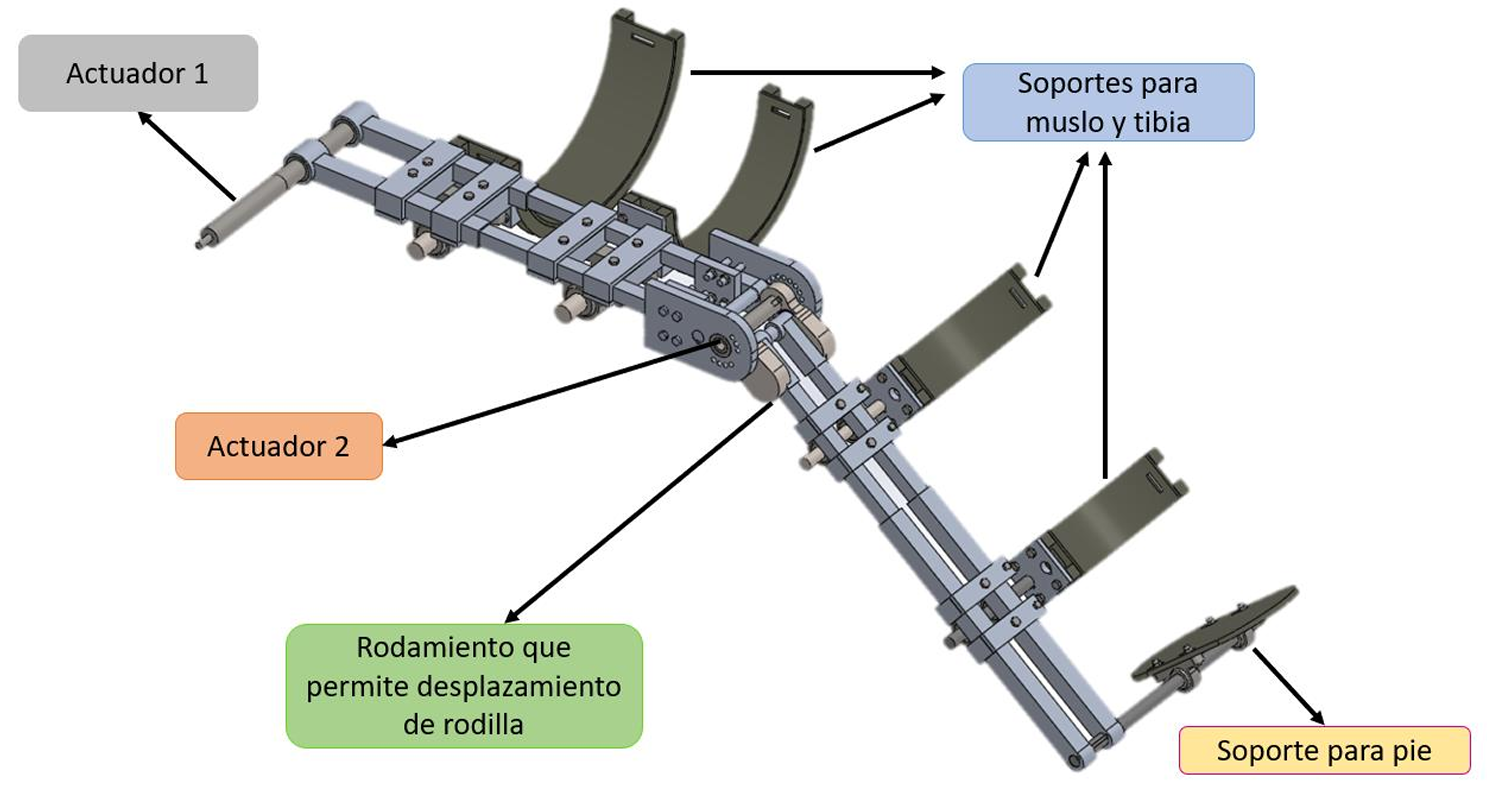
\includegraphics[width=1\linewidth]{imagenes/rehap_1.png}
    \caption{Sistema REHAP en CAD.}
    \label{fig:rh1}
\end{figure}


Los controladores no lineales pueden complementarse con herramientas adicionales, como observadores de estado y gobernadores de trayectoria, para mejorar la estimación de variables no medidas y ajustar las referencias de movimiento cuando se detectan condiciones que puedan afectar la estabilidad o la seguridad. Estas extensiones amplían la capacidad del sistema para adaptarse a cambios en la carga, en la velocidad del movimiento o en la respuesta mecánica del usuario. En la Figura \ref{fig:nl1} se muestra el lazo cerrado de control general.

\begin{figure}[H]
    \centering
    \begin{tikzpicture}[>=latex, thick, font=\small]
        \node (xd) at (0,0) {$x_d$};
        \node[draw, fill=blue!18, circle, minimum size=2.2em, inner sep=0pt]
            (sum) at (2.2,0) {};
        \node[font=\scriptsize] at (1.88, 0.30) {$+$};
        \node[font=\scriptsize] at (1.88,-0.35) {$-$};
        \node[draw, fill=blue!18, rectangle,
              minimum height=2.8em, minimum width=5em, align=center]
            (ctrl) at (5.2,0) {Control};
        \node[draw, fill=blue!18, rectangle,
              minimum height=2.8em, minimum width=5em, align=center]
            (plant) at (9.2,0) {Planta\\[2pt]o proceso};
        \node (y) at (12.2,0) {$y$};
        \node[draw, fill=blue!18, rectangle,
              minimum height=2.8em, minimum width=8em, align=center]
            (fb) at (5.7,-2.5) {Retroalimentación};
        \coordinate (spl) at (11.2,0);
        \draw[->] (xd)      -- (sum);
        \draw[->] (sum)     -- node[above]{$e$}  (ctrl);
        \draw[->] (ctrl)    -- node[above]{$u$}  (plant);
        \draw[->] (plant)   -- node[above]{$x$}  (spl);
        \draw[->] (spl)     -- (y);
        \draw[->] (spl)     |- (fb.east);
        \draw[->] (fb.west) -| (sum.south);
    \end{tikzpicture}
    \caption{Esquema general del lazo cerrado de control.}
    \label{fig:nl1}
\end{figure}


Los movimientos deben ser suaves, cíclicos y consistentes con patrones fisiológicos.

La precisión en la trayectoria es importante para evitar molestias o tensiones articulares.
En consecuencia, el controlador debe compensar dinámicas no modeladas, variaciones en rigidez articular y perturbaciones introducidas por el usuario o el entorno.

\subsubsection{Observadores de estado para sistemas de rehabilitación}

En muchos dispositivos de rehabilitación no es posible instrumentar el sistema con sensores adicionales debido a restricciones clínicas, estéticas, económicas o de seguridad; o simplemente, con la finalidad de mejorar la precisión del seguimiento de trayectoria, se requiere afinar la técnica de control.
Por ello, los observadores de estado surgen como herramientas auxiliares, a partir de mediciones mínimas, como posición articular, estos algoritmos estiman velocidades, torques e incluso perturbaciones externas \citep{slotine1991applied}. La Figura~\ref{fig:obs} ilustra el principio del observador de Luenberger —válido para sistemas lineales— donde la señal de corrección $L(y-\hat{y})$ cierra el lazo sobre el estimado $\hat{x}$. Para el sistema no lineal REHAP, este principio se generaliza mediante un \textbf{observador de alta ganancia} (HGO), cuya formulación se presenta en la Sección~\ref{sec:obs_hgo}.

\begin{figure}[H]
    \centering
    \begin{tikzpicture}[>=latex, thick, font=\small]
        \tikzset{
          blk/.style={draw, rectangle, minimum height=1.8em, minimum width=2.4em, align=center},
          sm/.style  ={draw, circle, minimum size=1.8em, inner sep=0pt}
        }
       
        \draw[dashed] (0.4,1.55) rectangle (7.8,3.3);
        \node[font=\scriptsize] at (1.5,3.1) {Sistema};
        \draw[dashed] (0.4,-1.9) rectangle (7.8,0.65);
        \node[font=\scriptsize] at (2.5,-1.7) {Observador de Luenberger};
        %% --- Sistema (y=2.5) ---
        \node      (u1) at (0,  2.5) {$u$};
        \node[blk] (B1) at (1.5,2.5) {$B$};
        \node[sm]  (s1) at (3.1,2.5) {};
        \node[blk] (i1) at (4.7,2.5) {$\int$};
        \node[blk] (C1) at (6.3,2.5) {$C$};
        \node[blk] (A1) at (3.9,1.9) {$A$};
        \coordinate (x1)    at (5.5,2.5);
        \coordinate (yfork) at (8.3,2.5);
        \node (yl) at (9.0,2.5) {$y$};
        \draw[->] (u1)--(B1);
        \draw[->] (B1)--(s1);
        \draw[->] (s1)-- node[above]{$\dot{x}$} (i1);
        \draw[->] (i1)-- node[above]{$x$} (x1) -- (C1);
        \draw[->] (C1)--(yfork)--(yl);
        \draw[->] (x1)--++(0,-0.6) -| (A1.east);
        \draw[->] (A1.west)--(3.1,1.9)--(s1.south);
        %% --- Observador (y=0) ---
        \node      (u2) at (0,  0) {$u$};
        \node[blk] (B2) at (1.5,0) {$B$};
        \node[sm]  (s2) at (3.1,0) {};
        \node[blk] (i2) at (4.7,0) {$\int$};
        \node[blk] (C2) at (6.3,0) {$C$};
        \node[blk] (A2) at (3.9,-1.3) {$A$};
        \node[blk] (L)  at (3.1,1.25) {$L$};
        \coordinate (xh)       at (5.5,0);
        \coordinate (yhatfork) at (8.3,0);
        \draw[->] (u2)--(B2);
        \draw[->] (B2)--(s2);
        \draw[->] (s2)-- node[above]{$\dot{\hat{x}}$} (i2);
        \draw[->] (i2)-- node[above]{$\hat{x}$} (xh) -- (C2);
        \draw[->] (C2)--(yhatfork);
        \node[font=\scriptsize,above] at (yhatfork) {$\hat{y}$};
        \draw[->] (xh)--++(0,-0.7) -| (A2.east);
        \draw[->] (A2.west)--(3.1,-1.3)--(s2.south);
        \draw[->] (L.south)--(s2.north);
        %% --- Unión de error e = y - ŷ ---
        \node[sm]  (se) at (8.3,1.25) {};
        \node[font=\tiny] at (8.55,1.55) {$+$};
        \node[font=\tiny] at (8.55,0.95) {$-$};
        \draw[->] (yfork)--(se.north);
        \draw[->] (yhatfork)--(se.south);
        \draw[->] (se.west)-- node[above]{$e$} (L.east);
    \end{tikzpicture}
    \caption{Observador de Luenberger: el término $L(y-\hat{y})$ cierra el lazo de corrección.}
    \label{fig:obs}
\end{figure}

Entre los observadores más utilizados se encuentran:
\begin{itemize}
    \item Observadores de Luenberger
    \item Observadores de alta ganancia 
    \item Observadores de perturbaciones
\end{itemize}





\subsubsection{Gobernadores de trayectoria}

Los gobernadores de trayectoria funcionan como una capa adicional de seguridad dentro del sistema de control. Su tarea principal es ajustar dinámicamente la referencia de movimiento en función de las condiciones presentes. Esto permite limitar aceleraciones, velocidades o amplitudes cuando el sistema detecta que se aproxima a una condición potencialmente riesgosa para el usuario.

Los gobernadores han sido estudiados como herramientas para garantizar que los sistemas respeten restricciones físicas, cinemáticas o de seguridad \citep{garone2017reference}. Su aplicación en robots de rehabilitación contribuye a prevenir movimientos bruscos, sobrecargas o alcances articulares no deseados, haciendo más segura la interacción humano–robot. En la Figura \ref{fig:gbt} se muestra el esquema general de un gobernador de trayectoria en lazo cerrado.

\begin{figure}[H]
    \centering
    \begin{tikzpicture}[>=latex, thick, font=\small]
        \node (r) at (0,0) {$r(t)$};
        \node[draw, fill=green!25, rectangle,
              minimum height=3em, minimum width=5.5em, align=center]
            (gov) at (2.9,0) {Reference\\governor};
        \node[draw, fill=blue!15, rectangle,
              minimum height=3em, minimum width=4.5em, align=center]
            (ctrl) at (6.5,0) {Controller};
        \node[draw, fill=blue!15, rectangle,
              minimum height=3em, minimum width=4em, align=center]
            (plant) at (10.0,0) {Plant};
        \node (z) at (12.3,0) {$z(t)$};
        \node (w) at (10.0,2.0) {$w(t)$};
        \coordinate (spl) at (11.3,0);
        \coordinate (bot1) at (10.0,-1.9);
        \coordinate (bot2) at (6.5,-1.9);
        %% flechas principales
        \draw[->] (r)    -- (gov);
        \draw[->] (gov)  -- node[above]{$v(t)$}  (ctrl);
        \draw[->] (ctrl) -- node[above]{$u(t)$}  (plant);
        \draw[->] (plant)-- (spl) -- (z);
        \draw[->] (w)    -- (plant.north);
        %% y(t) ∈ Y (salida inferior)
        \draw[->] (spl)  -- ++(0,-1.0) node[right]{$y(t)\in Y$};
        %% xp(t) retroalimentación
        \draw[->] (plant.south) -- (bot1) -- node[below]{$x_p(t)$} (bot2)
                  -- (ctrl.south);
    \end{tikzpicture}
    \caption{Esquema general de un gobernador de trayectoria.}
    \label{fig:gbt}
\end{figure}

\subsubsection{Arquitectura de control en cascada}

La integración de los componentes descritos se organiza en una arquitectura de control en cascada: múltiples lazos anidados operan en distintas escalas de tiempo, donde los lazos rápidos garantizan seguimiento de trayectoria y los lazos lentos aseguran seguridad clínica y adaptación terapéutica \citep{khalil2002nonlinear}. El principio de estabilidad en cascada establece que si cada subsistema es globalmente asintóticamente estable (GAS) de forma independiente y las soluciones son acotadas, el sistema completo es GAS \citep{khalil2002nonlinear}. Esto permite diseñar y validar cada nivel semiindependientemente, reduciendo la complejidad del análisis global.

En robótica de rehabilitación, las arquitecturas jerárquicas han demostrado ser eficaces para combinar objetivos de alto nivel (terapéuticos) con restricciones de bajo nivel (físicas y de seguridad), permitiendo que dispositivos como exoesqueletos adapten su comportamiento según el estado del paciente sin comprometer la estabilidad del lazo de control interno \citep{slotine1991applied}.

La Figura~\ref{fig:arch} presenta la arquitectura propuesta para REHAP con cinco capas funcionales:

\begin{figure}[H]
    \centering
    \begin{tikzpicture}[>=latex, thick, font=\small]
        \tikzset{lvl/.style={draw, rectangle, minimum height=2.6em,
                 minimum width=8.5em, align=center}}
        %% Bloques en cascada (eje central)
        \node[lvl, fill=purple!15] (agt) at (0, 7.5) {Agente\\Inteligente};
        \node[lvl, fill=green!20]  (gov) at (0, 5.5) {Gobernador\\de Referencia};
        \node[lvl, fill=blue!18]   (ctr) at (0, 3.5) {Control\\Backstepping};
        \node[lvl, fill=orange!15] (plt) at (0, 1.5) {Planta REHAP};
        \node[lvl, fill=yellow!25] (obs) at (0,-0.5) {Observador\\de Estado (HGO)};
        %% Cadena directa
        \draw[->] (agt) -- node[right]{$r(t)$}    (gov);
        \draw[->] (gov) -- node[right]{$v(t)$}    (ctr);
        \draw[->] (ctr) -- node[right]{$\tau(t)$} (plt);
        \draw[->] (plt) -- node[right]{$y(t)$}    (obs);
        %% Entradas externas (lado izquierdo)
        \node[align=center,font=\scriptsize] (thr) at (-3.0,7.5) {Objetivos\\clínicos};
        \node (Z)   at (-2.5,5.5) {$\mathcal{Z}$};
        \node (dst) at (-2.5,1.5) {$d(t)$};
        \draw[->] (thr)--(agt.west);
        \draw[->] (Z)  --(gov.west);
        \draw[->] (dst)--(plt.west);
        %% Retroalimentación x̂ (lado derecho)
        \draw[-]  (obs.east)  -- (3.0,-0.5);
        \draw[-]  (3.0,-0.5)  -- (3.0, 5.5);
        \draw[->] (3.0,3.5)   -- node[above,font=\scriptsize]{$\hat{x}$} (ctr.east);
        \draw[->] (3.0,5.5)   -- (gov.east);
        \node[font=\scriptsize,right] at (3.1,2.5) {$\hat{x}(t)$};
    \end{tikzpicture}
    \caption{Arquitectura de control en cascada propuesta para REHAP.}
    \label{fig:arch}
\end{figure}

\begin{itemize}
    \item \textbf{Agente Inteligente}: capa de supervisión que recibe los objetivos terapéuticos y genera la referencia de movimiento $r(t)$.
    \item \textbf{Gobernador de Referencia}: filtra $r(t)$ para producir la referencia segura $v(t)$, garantizando que el sistema respete el conjunto de restricciones $\mathcal{Z}$ \citep{garone2017reference}.
    \item \textbf{Control Backstepping}: ejecuta el seguimiento de $v(t)$ generando el torque $\tau(t)$, con garantías de estabilidad vía función de Lyapunov \citep{slotine1991applied}.
    \item \textbf{Planta REHAP}: sistema físico que recibe $\tau(t)$ y produce la salida medible $y(t)$, sujeta a perturbaciones $d(t)$ propias de la interacción humano-robot.
    \item \textbf{Observador de Alta Ganancia (HGO)}: reconstruye el vector de estados $\hat{x}(t)$ —incluyendo velocidades articulares y perturbaciones— a partir de $y(t)$, retroalimentando al controlador y al gobernador con garantías de convergencia exponencial.
\end{itemize}

En conjunto, el modelado dinámico, el control backstepping, el observador de estados, el gobernador de referencia y el agente inteligente ---integrados bajo la arquitectura en cascada--- constituyen los pilares del sistema propuesto, permitiendo un dispositivo de rehabilitación clínicamente seguro, robusto y adaptativamente eficiente.

\subsection{Inteligencia Artificial Embebida en Dispositivos Mecatrónicos}

El uso de inteligencia artificial en sistemas mecatrónicos ha avanzado hacia implementaciones capaces de ejecutarse directamente en hardware de bajo consumo mediante modelos compactos optimizados para tiempo real. Este enfoque permite dotar a los dispositivos de funciones de supervisión y adaptación sin depender de procesamiento externo. En robótica de rehabilitación, estas capacidades permiten ajustar parámetros operativos, detectar patrones de interacción variables entre usuarios y mejorar la seguridad mediante la identificación temprana de anomalías durante el movimiento asistido. La inteligencia artificial embebida se ha aplicado en control inteligente, clasificación de señales y supervisión autónoma, lo cual la hace adecuada para dispositivos terapéuticos con restricciones de cómputo.

\subsubsection{Agentes de IA ligeros para control y supervisión basados en LLM}

Los agentes construidos sobre modelos de lenguaje compactos permiten ejecutar razonamiento, toma de decisiones y tareas autónomas directamente en sistemas embebidos. El libro \textit{AI Agents in Action} describe arquitecturas modulares integradas por un planificador, un administrador de memoria, un evaluador de acciones y un componente de razonamiento, todos operando con modelos reducidos capaces de funcionar sin infraestructura externa \citep{lanham2024aiagents}. Esta estructura facilita el diseño de agentes que procesan información en tiempo real y generan respuestas adecuadas a condiciones variables de operación.


Los agentes basados en LLM pueden ejecutar tareas como:

\begin{itemize}
    \item análisis continuo de señales provenientes de encoders, IMUs o sensores de fuerza;
    \item detección de patrones anómalos en la trayectoria o el esfuerzo del usuario;
    \item ajuste de parámetros del controlador cuando se identifican desviaciones persistentes;
    \item activación de modos de seguridad tras evaluar riesgo de sobrecarga articular;
    \item clasificación de estados operativos del usuario para adaptar velocidad, amplitud o rigidez.
\end{itemize}

El empleo de agentes locales evita dependencia de servicios en la nube y reduce riesgos asociados a latencias variables o cortes de comunicación. Además, los agentes pueden integrarse como supervisores que validan las decisiones del controlador principal y emiten recomendaciones basadas en el estado histórico almacenado en la memoria del sistema. La literatura reciente muestra aplicaciones de agentes inteligentes en infraestructuras críticas y sistemas autónomos donde la toma de decisiones requiere fiabilidad y capacidad para identificar condiciones de falla \citep{feng2025integration, zhang2025intelligent}. Estos resultados respaldan el uso de agentes para reforzar la operación de robots de rehabilitación que deben responder ante variaciones del usuario y garantizar seguridad en la terapia.

Un agente LLM aporta una capa adicional de supervisión adaptativa sin comprometer los recursos del sistema. Su incorporación fortalece el monitoreo continuo, mejora la capacidad de detección temprana de desviaciones y favorece una operación más segura del dispositivo.


\subsection{Estado del Arte de Dispositivos Robóticos para Rehabilitación}

En la Tabla \ref{tab:estado} se presenta una clasificación de los distintos dispositivos y propuestas de robots de rehabilitación encontrados en la literatura, organizados según la articulación que abordan (rodilla, tobillo, combinado o general). Esta sistematización permite identificar con claridad las áreas de mayor investigación y aquellas que presentan vacíos o limitaciones. La relevancia de esta clasificación para nuestro estudio radica en que nos brinda un panorama comparativo, mostrando cómo la mayoría de los dispositivos se concentran en soluciones generales o en enfoques parciales (tobillo o rodilla), mientras que pocos trabajos integran de manera completa aspectos de control avanzado, facilidad de uso y posibilidad de personalización clínica.
\newpage

\begin{table}[htbp]
\centering
\scriptsize
\setlength{\tabcolsep}{3pt}
\renewcommand{\arraystretch}{1.1}
\begin{tabular}{p{.38\linewidth} p{.08\linewidth} p{.22\linewidth} p{.32\linewidth}}
\hline
\textbf{Trabajo} & \textbf{Año} & \textbf{Articulación} & \textbf{Principales características} \\
\hline
Prototipo para rehabilitación de miembros inferiores en lactantes hipotónicos \citep{garcia2022} & 2022 & Combinado & Robot paralelo; flexión–extensión cadera/rodilla/tobillo; enfocado en lactantes; proponen HMI y materiales más resistentes. \\
Modelo y simulación de un robot terapéutico para la rehabilitación de miembros inferiores \citep{revistaEIA}             & 2013  & General   & 3 GDL; par calculado con polinomio de Hurwitz; simulación en MATLAB; seguimiento de trayectorias. \\
TobiBot \citep{tobiBot2014}                 & 2014 & Tobillo   & 1 GDL; dorsiflexión/plantarflexión; interfaz tipo videojuego; seguridad básica. \\
Prototipo robotizado para la rehabilitación de lesiones de rodilla enfocado al fortalecimiento muscular \citep{unipamplona}            & 2022  & Rodilla   & Prototipo con IA/IoT; fortalecimiento; modelado CAD; supervisión web. \\
A Novel Hybrid Rehabilitation Robot for Upper and Lower Limbs Rehabilitation Training \citep{elsevierHybrid}     & 2014  & General   & Alcance en miembros superior e inferior; DC+DSP; realidad virtual; compacto/bajo costo. \\
Adaptive Patient-Cooperative Compliant Control of Lower Limb Rehabilitation Robot\citep{elsevierAdaptive} & 2024 & General & Pasivo; control adaptativo cooperativo; impedancia/admitancia; sensores de fuerza. \\
LegUp \citep{elsevierLegUp}                 & 2024  & General   & Robot paralelo para rehabilitación en cama; espacio de trabajo predefinido. \\
Admittance Controller complemented with real-time singularity avoidance for rehabilitation parallel robots \citep{elsevierAdmittance} & 2023 & General & Paralelo 4 GDL; seguimiento 3D (OptiTrack); evitación de singularidades. \\
A Novel Design of the Lower Limb Rehabilitation Robot \citep{ICMEAS2020}                   & 2020 & Combinado & Para adultos mayores; actuadores lineales y motores; modelado en SOLIDWORKS; verificación de torques. \\
Lower Limb Robotic Rehabilitation: Literature Review and Challenges \citep{journalRobotics} & 2011 & No aplica & Revisión: exoesqueletos y end-effector; control de posición/fuerza/señales biológicas; barreras de costo/evidencia. \\
Systematic Design of a Parallel Robotic System for Lower Limb Rehabilitation \citep{systematicDesign}  & 2020  & General   & Paralelogramo; flex–ext y abd–add; evita singularidades; sensores biomédicos. \\
Physiotherabot \citep{physiotherabot}       & 2011 & Rodilla (con cadera) & Flex–ext de cadera/rodilla y abd–add de cadera; control de impedancia + PID; interfaz clínica. \\
Model Analysis and Experimental Study of Lower Limb Rehabilitation Training Device Based on Gravity Balance \citep{MDPI2022}              & 2022 & Rodilla (con cadera) & Balance de gravedad con resortes; reducción de esfuerzo 87\% (rodilla) y 81\% (cadera). \\
Lower Limb Rehabilitation Robotics: Current Understanding and Technology. \citep{advancesRobotics} & 2021 & No aplica & Revisión: avances recientes; AR/IA; personalización; accesibilidad económica. \\
\hline
\end{tabular}
\caption{Clasificación por articulación (Rodilla, Tobillo, Combinado); se incluyen trabajos generales y revisiones.}
\label{tab:estado}
\end{table}


\subsubsection{Brecha identificada y aportación original}

El análisis del estado del arte revela que los dispositivos de rehabilitación de extremidad inferior se dividen en dos tendencias predominantes: (1) sistemas con control robusto y garantías formales de estabilidad pero sin capacidad de adaptación al estado cualitativo del paciente (p. ej., fatiga, dolor involuntario), y (2) sistemas con supervisión basada en IA pero sin fundamento matemático formal que garantice estabilidad ante perturbaciones biomecánicas no estructuradas. Ningún trabajo identificado integra simultáneamente: (a) un observador de estados con garantías de convergencia probadas por Lyapunov, (b) un gobernador de referencia con restricciones biomecánicas explícitas, (c) una arquitectura de agentes IA orquestadores capaz de interpretar señales cuantitativas del dispositivo y cualitativas del usuario en conjunto, y (d) un gemelo digital como entorno de co-simulación para la validación segura previa a la interacción humana —todo ello implementado y validado en un único sistema integrado de rehabilitación pasiva de extremidad inferior.

La aportación original de este trabajo al conocimiento consiste en el \textbf{diseño, implementación y validación pre-clínica de una arquitectura de control jerárquica que desacopla formalmente la seguridad dinámica de la inteligencia terapéutica} en un dispositivo robótico de rehabilitación. Esta arquitectura propone una solución al problema abierto de garantizar simultáneamente estabilidad matemática y adaptabilidad clínica en robots de rehabilitación pasiva, contribuyendo al campo de las Tecnologías Avanzadas con evidencia experimental replicable y métricas cuantificables de desempeño.

\newpage
\subsubsection{Contribuciones y colaboraciones previas del autor}

\paragraph{Artículos científicos}
\begin{itemize}
  \item \textbf{Primer autor en revista indexada por SECIHTI (Publicado)}.\\
  “J. E. Cervantes Reyes, M. D. L. Ángeles Alamilla Daniel, Ángel R. Lícona Rodriguez, and E. H. Ramirez Dominguez, “Comparative Analysis of Nonlinear Control Strategies for a Lower Limb Rehabilitation System”, Int. Journal of COP and Infor., vol. 16, no. 3, pp. 36–45, Jul. 2025."
 \item \textbf{Coautor en artículo JCR Q2 (Publicado)}. \\ 
“Identification and fuzzy control of the trajectory of a parallel robot: application to medical rehabilitation”, \emph{MDPI}, 2025. \\
Autores: Elihu H. Ramirez-Dominguez, J.G. Benítez-Morales, Jesus E. Cervantes-Reyes, M.A. Alamilla-Daniel, A.R. Licona-Rodríguez, Juan M. Xicotencatl-Pérez y Julio C. Ramos-Fernández.
\item \textbf{Coautor de poster (Publicado)}. \\
“Diseño de un sistema electromecánico para aplicaciones de rehabilitación de la extremidad superior”, Congreso CoNMiCyT, 2025. \\
Autores: Elihu Ramírez, Gerardo Benítez, Ángel Licona, Cesar Vilchis, Jesús Cervantes, Miguel Aguilera.


\item \textbf{Coautor de cartel (Publicado)}. \\
“Implementación de sistemas mecatrónicos en la 
rehabilitación física de extremidades”, Simposio Iberoamericano Multidisciplinario de Ciencias e Ingeniería, 2025. \\
Autores: Valdez García Yensy, Alamilla Daniel Ma. De Los Ángeles, Lícona Rodríguez Ángel Ricardo, Cortés Márquez Sandra Kristal y Cervantes Reyes Jesús Eduardo.
\end{itemize}

\paragraph{Ponencias y actividades académicas}
\begin{itemize}
  
  \item \textbf{Ponente}. “Sistemas mecatrónicos para rehabilitación física de extremidades”, \emph{Jornada Internacional de Energías, Mantenimiento y Mecatrónica}, Universidad Tecnológica de Tula-Tepeji, 2025.
  
  \item \textbf{Ponente}. Exposición de resultados parciales de tesis, \emph{Semana de la Mecatrónica}, Universidad Politécnica de Pachuca, 2025.
  \item \textbf{Evaluador de proyectos}. Proyectos integradores de estudiantes, \emph{EXPO SINERGÍA MANTRÓNICA}, Universidad Tecnológica de Tula-Tepeji, 2025.
\end{itemize}


\newpage

\section{Metodología}

La metodología se estructura conforme a los subsistemas fundamentales que integran el dispositivo mecatrónico de rehabilitación: el área de control y supervisión, el área mecánica y el área electrónica. Este enfoque es consistente con metodologías de diseño concurrente y co-diseño en robótica, donde los distintos subsistemas se desarrollan en paralelo para asegurar coherencia funcional, reducir iteraciones y favorecer la pertinencia del dispositivo en el ámbito clínico \citep{chhabra_holistic_2009, park_concurrent_2001, cruz_methodology_2017}. Asimismo, se consideran principios de diseño basado en modelos, co-simulación y gemelos digitales aplicados al desarrollo de robots de rehabilitación \citep{gil_model-based_2025, mazumder_next_2023}.

\subsection{Área de Control y Supervisión}

El desarrollo en esta área tiene como propósito mejorar la precisión, estabilidad y robustez del sistema mediante estrategias avanzadas de control, estimación y supervisión inteligente.

\subsubsection{Implementación del observador de estados}
\label{sec:obs_hgo}

El punto de partida es el modelo dinámico del sistema REHAP, formulado mediante la ecuación de Euler–Lagrange para un robot de $n=2$ grados de libertad:

\begin{equation}
    M(q)\ddot{q} + C(q,\dot{q})\dot{q} + G(q) + F(\dot{q}) = \tau + \tau_d,
    \label{eq:dinamica}
\end{equation}

\noindent donde $q,\dot{q},\ddot{q}\in\mathbb{R}^{2}$ son los vectores de posición, velocidad y aceleración articular; $M(q)\in\mathbb{R}^{2\times 2}$ es la matriz de inercia (simétrica definida positiva); $C(q,\dot{q})\in\mathbb{R}^{2\times 2}$ contiene los términos de Coriolis y fuerzas centrífugas; $G(q)\in\mathbb{R}^{2}$ es el vector de fuerzas gravitacionales; $F(\dot{q})\in\mathbb{R}^{2}$ modela la fricción viscosa y seca; $\tau\in\mathbb{R}^{2}$ es el vector de torques de control; y $\tau_d\in\mathbb{R}^{2}$ representa perturbaciones externas debidas a la interacción con el usuario.

Expresando \eqref{eq:dinamica} en espacio de estados con $x=[q^{\top},\dot{q}^{\top}]^{\top}\in\mathbb{R}^{4}$, se obtiene la representación:

\begin{equation}
    \dot{x} = f(x) + g(x)\,u + d(t), \qquad y = \mathbf{H}x,
    \label{eq:estadoesp}
\end{equation}

\noindent con $u=\tau$ y $\mathbf{H}=[I_{2}\;0_{2}]\in\mathbb{R}^{2\times 4}$ la matriz de salida (donde $I_{2},0_{2}\in\mathbb{R}^{2\times 2}$), que refleja que únicamente la posición articular $q$ es medible mediante encoders incrementales. Para evitar ambigüedad con la matriz de Coriolis $C(q,\dot{q})$, la matriz de salida se denota $\mathbf{H}$ en todo el documento. Particionando $x=[x_1^{\top},x_2^{\top}]^{\top}$ con $x_1=q$ y $x_2=\dot{q}$, los campos vectoriales se definen como:
\begin{equation}
    f(x) = \begin{bmatrix} x_2 \\ -M^{-1}(x_1)\bigl(C(x_1,x_2)\,x_2 + G(x_1) + F(x_2)\bigr) \end{bmatrix},\quad
    g(x) = \begin{bmatrix} 0_{2\times 2} \\ M^{-1}(x_1) \end{bmatrix}\in\mathbb{R}^{4\times 2},
    \label{eq:fg}
\end{equation}
y $d(t)=\bigl[0_{2}^{\top},\;(M^{-1}(q)\,\tau_d)^{\top}\bigr]^{\top}\in\mathbb{R}^{4}$ concentra las perturbaciones sobre la dinámica de velocidad.

Se diseñará un \textbf{observador de alta ganancia} para reconstruir $\dot{q}$ y estimar $\tau_d$ en tiempo real. El observador propuesto tiene la forma:

\begin{equation}
    \dot{\hat{x}} = f(\hat{x}) + g(\hat{x})\,u + L\bigl(y - \mathbf{H}\hat{x}\bigr),
    \label{eq:observador}
\end{equation}

\noindent donde $\hat{x}\in\mathbb{R}^{4}$ es el vector de estados estimados y $L\in\mathbb{R}^{4\times 2}$ es la ganancia del observador. A diferencia del caso lineal —donde se requiere que $(A-L\mathbf{H})$ sea Hurwitz— la estabilidad del error de observación $e = x - \hat{x}\in\mathbb{R}^{4}$ se analiza mediante la función candidata de Lyapunov $V(e)=e^{\top}Pe$, con $P=P^{\top}>0$. La dinámica del error resulta:
\begin{equation}
    \dot{e} = \bigl[f(x)-f(\hat{x})\bigr] + \bigl[g(x)-g(\hat{x})\bigr]u - L\mathbf{H}\,e + d(t),
    \label{eq:error_obs}
\end{equation}
donde $[f(x)-f(\hat{x})]$ es Lipschitz en $e$ sobre una región compacta de operación. Se elige $L$ tal que $\dot{V}(e)=\dot{e}^{\top}Pe+e^{\top}P\dot{e}<0$ a lo largo de las trayectorias del error, asegurando convergencia exponencial $\|e(t)\|\leq\beta\,\|e(0)\|\,e^{-\lambda t}$ con $\beta,\lambda>0$. El análisis de observabilidad local del sistema alrededor de la trayectoria de operación será verificado previo a la implementación. Adicionalmente, se considerará la atenuación del \textit{peaking phenomenon} propio de los HGO mediante saturación de la ganancia $L$ durante el transitorio inicial.

La estimación se apoyará en la instrumentación disponible: encoders incrementales (posición articular), sensores de corriente (inferencia de esfuerzo en actuadores) y sensores inerciales (información cinemática complementaria). Esto permite reconstruir $\dot{q}$ y $\tau_d$ sin sensores adicionales que compliquen la operación clínica.

\subsubsection{Integración del gobernador de trayectoria}

El gobernador de referencia actúa como capa de seguridad entre la trayectoria prescrita $r(t)$ y la referencia efectivamente enviada al controlador $v(t)$. El sistema opera en tiempo discreto con período de muestreo $T_s$, y se define el vector de estado extendido $z(t)=\bigl(q(t),\dot{q}(t),\tau(t)\bigr)\in\mathbb{R}^{6}$, donde los índices $t+k$ corresponden a $k$ pasos de tiempo de tamaño $T_s$. En cada instante, el gobernador resuelve el siguiente problema de factibilidad escalar:

\begin{equation}
    \kappa^{*}(t) = \max\bigl\{\kappa \in [0,1] \;\big|\; \text{para todo } k\in\{0,\ldots,N\}:\; z(t+k)\in\mathcal{Z}\bigr\},
    \label{eq:governor}
\end{equation}
\begin{equation}
    v(t) = v(t-1) + \kappa^{*}(t)\,\bigl[r(t) - v(t-1)\bigr],
    \label{eq:governor2}
\end{equation}

\noindent donde $z(t)$ es la trayectoria predicha del sistema a lazo cerrado y $\mathcal{Z}$ es el conjunto de restricciones de seguridad biomecánica, definido como:

\begin{equation}
    \mathcal{Z} = \bigl\{(q,\dot{q},\tau) \;\big|\; q_{\min}\leq q \leq q_{\max},\; |\dot{q}|\leq \dot{q}_{\max},\; |\tau|\leq \tau_{\max}\bigr\},
    \label{eq:Zset}
\end{equation}

\noindent con $q_{\min}$, $q_{\max}$ determinados por los rangos fisiológicos articulares seguros, $\tau_{\max}$ por la capacidad nominal de los actuadores, y $N$ el horizonte de predicción finito, seleccionado en función de la dinámica del sistema y el periodo de muestreo. Cuando $\kappa^{*}=1$ el gobernador es transparente; cuando $\kappa^{*}<1$ suaviza la referencia para mantener al sistema dentro de $\mathcal{Z}$, previniendo movimientos bruscos o sobrecargas \citep{garone2017reference}. La predicción de $z(t+k)$ se realizará utilizando el modelo del gemelo digital descrito en la sección siguiente.

\subsubsection{Construcción del gemelo digital}
\label{sec:gemelo_digital}

El gemelo digital (DT) constituye una réplica virtual dinámica del dispositivo REHAP que opera en paralelo y en tiempo real con el sistema físico. A diferencia de un modelo de simulación convencional, el DT se actualiza continuamente con datos sensoriales reales, manteniendo sincronización activa entre el estado virtual $\hat{x}_{DT}$ y el estado medido $x$. Esto le permite desempeñar tres roles simultáneos en la arquitectura de control: (1)~predictor de trayectorias para el gobernador de referencia, (2)~detector de anomalías mediante análisis de residuos, y (3)~entorno seguro de validación previa a la interacción humana \citep{gil_model-based_2025, mazumder_next_2023}.

\paragraph{Modelo dinámico virtual.}
El gemelo resuelve en tiempo real la misma ecuación de Euler–Lagrange del sistema físico \eqref{eq:dinamica} sobre un entorno de cómputo sin restricciones de seguridad física:

\begin{equation}
    M(\hat{q}_{DT})\ddot{\hat{q}}_{DT}
    + C(\hat{q}_{DT},\dot{\hat{q}}_{DT})\dot{\hat{q}}_{DT}
    + G(\hat{q}_{DT}) + F(\dot{\hat{q}}_{DT}) = \tau_{DT},
    \label{eq:dt_dinamica}
\end{equation}

\noindent donde $\hat{q}_{DT}\in\mathbb{R}^{2}$ son las coordenadas generalizadas del gemelo, $\dot{\hat{q}}_{DT},\ddot{\hat{q}}_{DT}\in\mathbb{R}^{2}$ sus derivadas primera y segunda, y $\tau_{DT}=\tau(t)\in\mathbb{R}^{2}$ es el torque de control aplicado simultáneamente al sistema físico y al gemelo. El vector de estado del gemelo se define como $\hat{x}_{DT}=[\hat{q}_{DT}^{\top},\dot{\hat{q}}_{DT}^{\top}]^{\top}\in\mathbb{R}^{4}$, con salida virtual $\hat{y}_{DT}(t)=\mathbf{H}\hat{x}_{DT}(t)\in\mathbb{R}^{2}$. Los parámetros dinámicos $M$, $C(q,\dot{q})$, $G$, $F$ son identificados experimentalmente y actualizados mediante estimación paramétrica en línea para mantener fidelidad con el sistema real.

\paragraph{Sincronización y detección de anomalías.}
La fidelidad del DT depende de la corrección continua entre su salida y la medición real. Se define el \textit{residuo de sincronización}:

\begin{equation}
    \rho(t) = y(t) - \hat{y}_{DT}(t) = \mathbf{H}\bigl(x(t)-\hat{x}_{DT}(t)\bigr)\in\mathbb{R}^{2},
    \label{eq:residuo}
\end{equation}

\noindent donde $y(t)=\mathbf{H}x(t)\in\mathbb{R}^{2}$ es la salida medida del sistema físico y $\rho_{\max}\in\mathbb{R}_{>0}$ es el umbral de sincronización, ajustado en función de la incertidumbre paramétrica aceptable del modelo. Cuando $\|\rho(t)\|>\rho_{\max}$, se activa una rutina de re-identificación paramétrica. Simultáneamente, el agente técnico de IA analiza la evolución temporal de $\rho(t)$ para detectar anomalías mecánicas —desgaste, desalineación, espasmos del usuario— que no serían detectables únicamente mediante encoders.

\paragraph{Predicción para el gobernador.}
Ante cada solicitud de referencia $r(t)$, el gemelo simula $N$ pasos hacia adelante con el estado actual $\hat{x}_{DT}(t)$ y el torque propuesto, generando la secuencia $z(t+k)$, $k=0,\ldots,N$, requerida por la \cref{eq:governor}. Esto elimina la necesidad de resolver iterativamente el sistema físico real y reduce la latencia del ciclo de gobernanza.

La Figura~\ref{fig:dt} ilustra la arquitectura del gemelo digital integrada al sistema REHAP.

\begin{figure}[H]
    \centering
    \begin{tikzpicture}[>=latex, thick, font=\small]
        \tikzset{
            blk/.style={draw, rectangle, rounded corners=2pt,
                        minimum height=2.8em, minimum width=7.5em, align=center},
            sm/.style ={draw, circle, minimum size=2.2em, inner sep=0pt}
        }
        %% ---- Bloques ----
        \node[blk, fill=orange!20] (phy) at (0,   4.0) {Sistema Físico\\REHAP};
        \node[blk, fill=cyan!20]   (dt)  at (0,   0.0) {Gemelo Digital\\(virtual)};
        \node[sm]                  (sum) at (5.5,  2.0) {};
        \node[font=\tiny] at (5.08, 2.50) {$+$};
        \node[font=\tiny] at (5.08, 1.50) {$-$};
        \node[blk, fill=red!10]    (agt) at (9.5,  2.0) {Agente IA\\(anomalías)};
        \node[blk, fill=green!20]  (gov) at (0,  -3.0) {Gobernador\\(predicciones)};
        %% ---- Entrada u(t) ----
        \node (u) at (-4.2, 2.0) {$u(t)$};
        \coordinate (split) at (-2.8, 2.0);
        \draw[-]  (u) -- (split);
        \fill     (split) circle (2pt);
        \draw[->] (split) |- (phy.west);
        \draw[->] (split) |- (dt.west);
        %% ---- y(t): físico -> sumador ----
        \coordinate (yfork) at (2.5, 4.0);
        \draw[-]  (phy.east) -- (yfork);
        \fill     (yfork) circle (1.5pt);
        \node[above, font=\scriptsize] at (yfork) {$y(t)$};
        \draw[->] (yfork) -| (sum.north);
        %% ---- ŷ_DT(t): gemelo -> sumador ----
        \coordinate (dtfork) at (2.5, 0.0);
        \draw[-]  (dt.east) -- (dtfork);
        \fill     (dtfork) circle (1.5pt);
        \node[below, font=\scriptsize] at (dtfork) {$\hat{y}_{DT}(t)$};
        \draw[->] (dtfork) -| (sum.south);
        %% ---- rho(t): sumador -> agente IA ----
        \draw[->] (sum.east) -- node[above]{$\rho(t)$} (agt.west);
        %% ---- z(t+k): gemelo -> gobernador ----
        \draw[->] (dt.south) -- node[right, font=\scriptsize]{$z(t+k)$} (gov.north);
        %% ---- Sincronización bilateral ----
        \draw[<->, dashed, gray!60]
            (phy.west) -- ++(-0.9, 0) |-
            node[left, font=\scriptsize, pos=0.5]{sync}
            (dt.west);
    \end{tikzpicture}
    \caption{Gemelo digital integrado al sistema REHAP: sincronización con el sistema físico, generación del residuo $\rho(t)$ para el agente IA y predicción de $z(t+k)$ para el gobernador.}
    \label{fig:dt}
\end{figure}

\paragraph{Plataforma de co-simulación.}
La implementación se realizará sobre una arquitectura de co-simulación donde el modelo dinámico virtual opera en MATLAB/Simulink con Simscape Multibody, interfazado con el microcontrolador del prototipo mediante comunicación serie de baja latencia. Los parámetros del modelo se actualizan con frecuencia $f_{\mathrm{sync}} < f_c$ (siendo $f_c$ la frecuencia del lazo de control), garantizando que la carga computacional del gemelo no comprometa el desempeño en tiempo real del controlador principal.

\subsubsection{Protocolos de seguridad y mecanismos de \textit{hard stop}}

La operación del dispositivo incorporará un conjunto de mecanismos redundantes de seguridad destinados a prevenir movimientos no deseados y proteger al usuario en todo momento. El sistema contará con cuatro niveles de detención:

\begin{itemize}
    \item \textbf{Corte físico de corriente}. Será el mecanismo prioritario. El terapeuta dispondrá de un interruptor dedicado para desenergizar inmediatamente el sistema ante cualquier situación crítica.
    
    \item \textbf{Paro de emergencia lógico}. Tanto el paciente como el terapeuta tendrán acceso a un botón de paro accesible en todo momento. Este mecanismo detendrá la rutina en ejecución y ordenará el retorno controlado a la posición inicial del sistema.
    
    \item \textbf{Detención por parte del observador}. Cuando el observador identifique señales compatibles con inestabilidad, aceleraciones no previstas, incrementos súbitos de corriente o cualquier patrón asociado a una falla, ejecutará una parada segura y ordenará el retorno a casa.
    
    \item \textbf{Detención por el agente de IA}. El agente orquestador analizará patrones temporales en la interacción y señales de desempeño. Si detecta desviaciones repetitivas, resistencia involuntaria o comportamiento atípico del actuador, activará un protocolo seguro deteniendo el movimiento y regresando al estado inicial.
\end{itemize}

Estos mecanismos permiten cubrir fallas físicas, lógicas, dinámicas y predictivas, ofreciendo un marco de seguridad adecuado para futuras evaluaciones con usuarios.


\subsubsection{Arquitectura de agentes de inteligencia artificial}

La supervisión inteligente del sistema incluirá una arquitectura de agentes IA basada en frameworks orientados a la colaboración entre agentes, como \textit{CrewAI}. Esta arquitectura permitirá procesar simultáneamente información cuantitativa del dispositivo y datos cualitativos proporcionados por el usuario, facilitando decisiones autónomas relacionadas con la seguridad y el desempeño de la terapia.

El diseño contemplará al menos tres agentes:

\begin{itemize}
    \item \textbf{Agente técnico del sistema}. Analizará señales provenientes de la instrumentación, como encoders, sensores de corriente, parámetros cinemáticos y registros de esfuerzo. Su función será generar un reporte cuantitativo capaz de identificar incrementos anómalos en torque, perturbaciones, desalineaciones o cualquier variación relevante en la dinámica mecánica.

    \item \textbf{Agente cualitativo del paciente}. Procesará información subjetiva proporcionada por el usuario mediante una interfaz de retroalimentación. Esta interfaz consistirá en un control accesible para el paciente, ya sea botones, un deslizador o una perilla, mediante el cual podrá indicar niveles de cansancio, molestia o dolor. El agente transformará esta señal cualitativa en un indicador interpretable para la supervisión del sistema.

    \item \textbf{Agente orquestador}. Recibirá los reportes generados por los dos agentes anteriores y tomará decisiones respecto al avance de la sesión terapéutica. El orquestador podrá aplicar ajustes automáticos como reducción de velocidad, disminución de amplitud de referencia o ejecución de un paro seguro con retorno a la posición inicial cuando los reportes indiquen condiciones desfavorables.
\end{itemize}

Esta estructura permitirá que las decisiones del sistema no dependan exclusivamente de la dinámica mecánica o del desempeño del paciente, sino de la integración simultánea de ambos tipos de información. La arquitectura también fortalecerá los mecanismos de seguridad al complementar los protocolos de detención descritos anteriormente, proporcionando una capa adicional basada en análisis temporal y patrones de comportamiento.

\subsection{Validación experimental y pre-clínica}

\subsubsection{Evaluación integral del sistema}
Una vez integradas las mejoras en control, mecánica y electrónica, se realizará una evaluación completa midiendo métricas de seguimiento de trayectoria, estabilidad del control, robustez ante perturbaciones y seguridad operativa.

\subsubsection{Pruebas con pacientes sanos}
Se realizarán pruebas controladas con sujetos sanos bajo supervisión clínica, con el objetivo de ajustar parámetros, evaluar comodidad y verificar la operación segura del dispositivo, siguiendo metodologías establecidas en robótica de rehabilitación \citep{cruz_methodology_2017}. El protocolo experimental contemplará los siguientes elementos:

\begin{itemize}
    \item \textbf{Tamaño de muestra}: $n \geq 10$ participantes sanos (estimación inicial por potencia estadística, sujeta a ajuste tras análisis formal).
    \item \textbf{Criterios de inclusión}: adultos de 18 a 45 años, sin lesiones musculoesqueléticas activas en extremidad inferior, sin contraindicaciones neurológicas, con consentimiento informado firmado.
    \item \textbf{Criterios de exclusión}: embarazo, implantes metálicos en el miembro inferior, trastornos de coagulación, hipertensión no controlada o cualquier condición que contraindique ejercicio pasivo asistido.
    \item \textbf{Métricas de evaluación}: RMSE y error máximo de seguimiento de trayectoria articular (°), suavidad del movimiento (jerk normalizado), tiempos de reacción de los mecanismos de detención de emergencia, y escala subjetiva de comodidad (EVA 0–10).
    \item \textbf{Ética}: el protocolo será sometido al Comité de Bioética Institucional de la Universidad Politécnica de Pachuca previo al inicio de las pruebas con usuarios. No se realizará ninguna sesión con sujetos humanos sin contar con la aprobación formal correspondiente.
\end{itemize}

\newpage


\subsection{Cronograma de actividades}
\begin{table}[H]
    \centering
    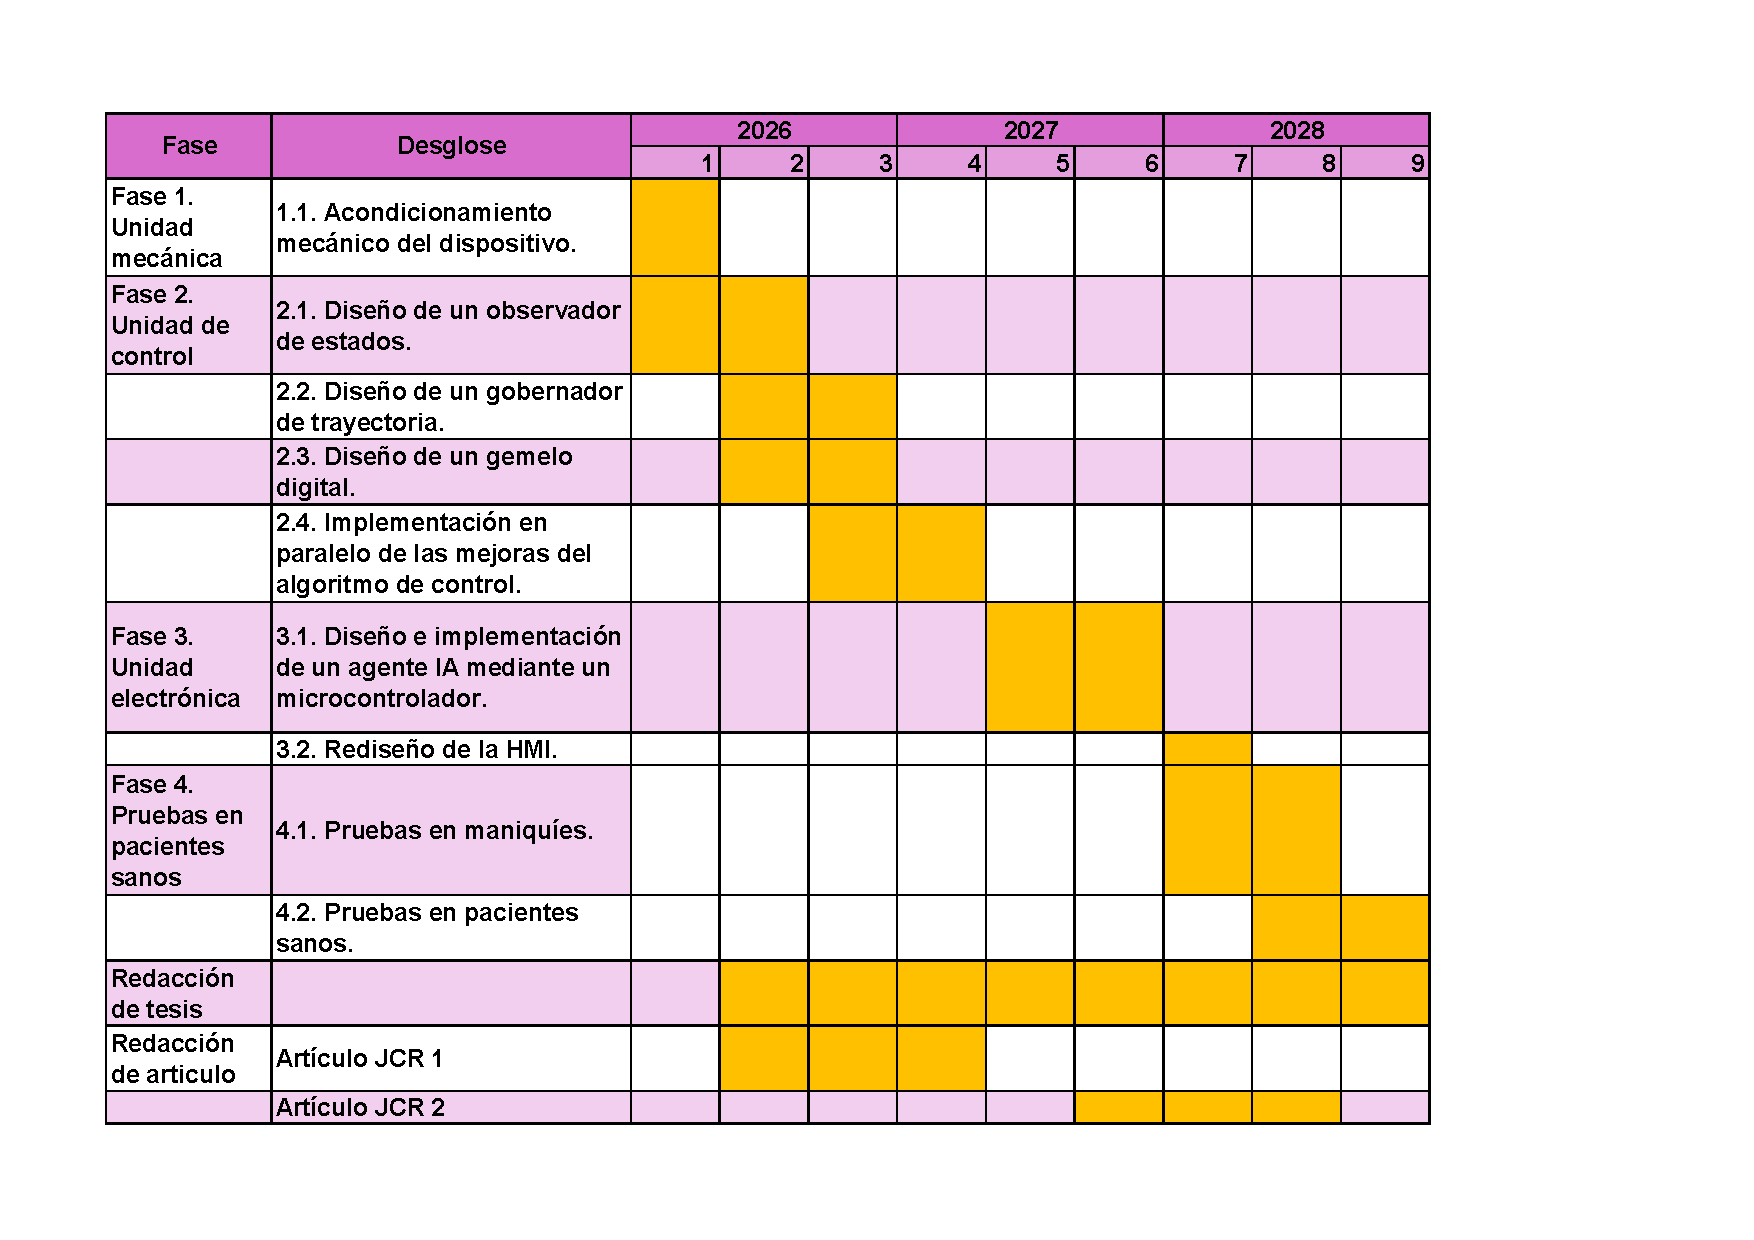
\includegraphics[width=1.2\linewidth]{imagenes/cronograma.pdf}
    \caption{Cronograma de actividades.}
    \label{tab:cronograma}
\end{table}

\subsection{Productos esperados}
\begin{itemize}
    \item Artículo JCR en relación con la implementación de un agente IA en el sistema REHAP.
    \item Artículo JCR en relación con la validación del sistema REHAP en sujetos sanos.
\end{itemize}

\newpage
\begin{thebibliography}{99}

\bibitem[Chhabra \& Emami(2009)]{chhabra_holistic_2009}
Chhabra, R., \& Emami, M. (2009). \textit{A holistic approach to concurrent engineering and its application to robotics}. Journal of Robotics.

\bibitem[Park(2001)]{park_concurrent_2001}
Park, J. H. (2001). \textit{Concurrent-design optimization of mechanical structure and control}. In ASME Design Engineering Technical Conferences.

\bibitem[Cruz-Martínez et al.(2017)]{cruz_methodology_2017}
Cruz-Martínez, E., et al. (2017). \textit{Methodology for the design of rehabilitation robots: Application in an upper limb exoskeleton}. Revista Iberoamericana de Automática e Informática Industrial.

\bibitem[Gil et al.(2025)]{gil_model-based_2025}
Gil, A., et al. (2025). \textit{A model-based approach for co-simulation-driven digital twins in robotics}. Robotics and Autonomous Systems.

\bibitem[Mazumder et al.(2023)]{mazumder_next_2023}
Mazumder, O., et al. (2023). \textit{Towards next generation digital twin in robotics}. Heliyon.

\bibitem[Spong et al.(2006)]{spong2006robot}
Spong, M. W., Hutchinson, S., \& Vidyasagar, M. (2006). \textit{Robot Modeling and Control}. Wiley.

\bibitem[Siciliano et al.(2010)]{siciliano2010robotics}
Siciliano, B., Sciavicco, L., Villani, L., \& Oriolo, G. (2010). \textit{Robotics: Modelling, Planning and Control}. Springer.

\bibitem[Khalil(2002)]{khalil2002nonlinear}
Khalil, H. K. (2002). \textit{Nonlinear Systems} (3rd ed.). Prentice Hall.

\bibitem[Slotine \& Li(1991)]{slotine1991applied}
Slotine, J. J. E., \& Li, W. (1991). \textit{Applied Nonlinear Control}. Prentice Hall.

\bibitem[Garone et al.(2017)]{garone2017reference}
Garone, E., Di Cairano, S., \& Kolmanovsky, I. (2017). Reference and command governors for systems with constraints: A survey on theory and applications. \textit{Automatica}, 75, 306--328.

\bibitem[Reyes et al.(2025)]{reyes2025comparative}
Reyes, J. E., Alamilla, M., Rodríguez, Á., \& Domínguez, E. (2025). Comparative analysis of nonlinear control strategies for a lower limb rehabilitation system. \textit{International Journal of Combinatorial Optimization Problems and Informatics}, 16(3), 36--45. https://doi.org/10.61467/2007.1558.2025.v16i3.1129


\bibitem[Martínez et al.(2014)]{tobiBot2014}
Guzmán Valdivia, C. H., Carrera Escobedo, J. L., Blanco Ortega, A., Oliver Salazar, M. A., \& Gómez Becerra, F. A. (2014).
\textit{Diseño y control de un sistema interactivo para la rehabilitación de tobillo: TobiBot}.
Ingeniería Mecánica, Tecnología y Desarrollo, 5(1), 255–264.


\bibitem[Araque(2022)]{unipamplona}
Araque Isidro, J. E. (2022).
\textit{Diseño y control de un prototipo robotizado para la rehabilitación de lesiones de rodilla enfocado al fortalecimiento muscular}.
Universidad de Pamplona – Facultad de Ingenierías y Arquitectura. Tesis de Maestría.



\bibitem[Akdoğan \& Adli(2011)]{physiotherabot}
Akdoğan, E., \& Adli, M. A. (2011).
The design and control of a therapeutic exercise robot for lower limb rehabilitation (Physiotherabot).
\textit{Mechatronics}, 21(3), 509--522.
https://doi.org/10.1016/j.mechatronics.2011.01.005



\bibitem[Lanham(2024)]{lanham2024aiagents}
Lanham, M. (2024). \textit{AI Agents in Action}. Manning Publications.

\bibitem[Feng et al.(2025)]{feng2025integration}
Feng, J., Yu, T., Zhang, K., \& Cheng, L. (2025). Integration of multi-agent systems and artificial intelligence in self-healing subway power supply systems: Advancements in fault diagnosis, isolation and recovery. \textit{Processes}, 13(4), 1144. https://doi.org/10.3390/pr13041144

\bibitem[Zhang et al.(2025)]{zhang2025intelligent}
Zhang, H., Ran, H., \& Tang, X. (2025). Intelligent agents for software engineering: A systematic literature review. \textit{ACM Transactions on Software Engineering and Methodology}. (En prensa).

\bibitem[García \& Lugo-González(2022)]{garcia2022}
García, M., \& Lugo-González, E. (2022). Prototipo para rehabilitación de miembros inferiores en lactantes hipotónicos. \textit{Padil: Boletín Científico de Ciencias Básicas e Ingenierías del ICBI}.
\bibitem[López \& Pérez(2013)]{revistaEIA}
López, M., \& Pérez, A. (2013). Modelo y simulación de un robot terapéutico para la rehabilitación de miembros inferiores. \textit{Revista Ingeniería Biomédica de la EIA}.

\bibitem[Khor et al.(2014)]{elsevierHybrid}
Khor, K. X., Pérez-Zepeda, I. D., Peña, I., \& Lee, G. (2014).
A novel hybrid rehabilitation robot for upper and lower limbs rehabilitation training.
\textit{Procedia Computer Science}, 42, 293--300.
https://doi.org/10.1016/j.procs.2014.11.065

\bibitem[Wang et al.(2024)]{elsevierAdaptive}
Wang, Y., Li, X., Chen, H., \& Zhao, L. (2024).
Adaptive patient-cooperative compliant control of lower limb rehabilitation robot.
\textit{ISA Transactions}. 
https://doi.org/10.1016/j.isatra.2023.11.004

\bibitem[Birlescu et al.(2024)]{elsevierLegUp}
Birlescu, I., Tohănean, N., Vaida, C., Gherman, B., Negură, D., Horsiă, A., Tucan, P., Condurache, D., \& Pisla, D. (2024).
Modeling and analysis of a parallel robotic system for lower limb rehabilitation with predefined operational workspace.
\textit{Mechanism and Machine Theory}. Advance online publication.
https://doi.org/10.2139/ssrn.4753036



\bibitem[Pulloquinga et al.(2023)]{elsevierAdmittance}
Pulloquinga, J. L., Escarabajal, R. J., Vallés, M., Díaz-Rodríguez, M., Mata, V., \& Valera, Á. (2023).  
Admittance controller complemented with real-time singularity avoidance for rehabilitation parallel robots.  
\textit{Mechatronics}, 94, 103017. https://doi.org/10.1016/j.mechatronics.2023.103017



\bibitem[Zhang et al.(2020)]{ICMEAS2020}
Zhang, H., Li, Y., Wang, Q., \& Chen, X. (2020).  
A novel design of the lower limb rehabilitation robot.  
En \textit{Proceedings of the 2020 6th International Conference on Mechanical Engineering and Automation Science (ICMEAS)} (pp. 45--50). IEEE.
https://doi.org/10.1109/ICMEAS51072.2020.00015


\bibitem[Díaz et al.(2011)]{journalRobotics}
Díaz, I., Gil, J. J., \& Sánchez, E. (2011).
Lower limb robotic rehabilitation: Literature review and challenges.
\textit{Journal of Robotics}, 2011, Article 759764.
https://doi.org/10.1155/2011/759764



\bibitem[Carbone(2020)]{systematicDesign}
Carbone, G. (2020).
Systematic design of a parallel robotic system for lower limb rehabilitation.
\textit{IEEE Access}, 8, 111758–111770. https://doi.org/10.1109/ACCESS.2020.3000644



\bibitem[Wang et al.(2022)]{MDPI2022}
Wang, J., Kan, Y., Zhang, T., Zhang, Z., \& Xu, M. (2022).  
Model analysis and experimental study of lower limb rehabilitation training device based on gravity balance.  
\textit{Machines, 10}(7), 514. https://doi.org/10.3390/machines10070514



\bibitem[Bhardwaj et al.(2021)]{advancesRobotics}
Bhardwaj, S., Khan, A. A., \& Muzammil, M. (2021).
Lower limb rehabilitation robotics: The current understanding and technology.
\textit{Work: A Journal of Prevention, Assessment \& Rehabilitation, 69}(3), 775–793.
https://doi.org/10.3233/WOR-205012

\end{thebibliography}

\end{document}
